

\section{Periodic solution}
\label{sec:periodic-solution}

Before turning to the methods themselves, a few concepts will be revisited.
Computing the periodic solution of a nonlinear system means searching for a
solution $\bm x$ to

\begin{equation}
    \label{eq:per_eom}
  \bm M \ddot{\bm x}(t) + \bm C \dot{\bm x}(t) + \bm K \bm x(t) +
  \bm f_{nl} \left( \bm x(t), \dot{ \bm x}(t) \right) = \bm p (t)
\end{equation}
that satisfies a periodicity condition
\begin{equation}
  \label{eq:per_condtion}
  \bm x(t+T) = \bm x(t)
\end{equation}
where $T$ is the period. This is a boundary value problem(BVP). By periodic
solution, steady state conditions are implied. Stability of the periodic
solution will also be addressed.


There are at least three ways to describe such a periodic solution.

\begin{itemize}
\item Provide initial condition $\left[\bm x_0, \dot{\bm x}_0 \right]$ and the
  period $T$. Then do time integration over $T$.
\item Use Fourier series and the period $T$
\item Use piecewise polynomial functions and the period $T$
\end{itemize}

In this section methods for finding the first and second representations of a
periodic solution is described. They are denoted the shooting method and
harmonic balance method respectively. The third and not covered is called
Orthogonal collocation. The shooting method is used as part of calculating NNMs
and harmonic balance is used for bifurcation analysis. Both methods could be
used for either tasks, but as they are popular it is instructive to present
both.

\subsection{Shooting method}
\label{sec:shooting_method}

With the shooting method one finds, in an iterative way, the initial state $\bm
z = [\bm x, \dot{\bm x}]^T$ and period $T$ that describes a periodic
motion \autocite{nayfeh2008applied}.

One start by guessing on a periodic steady state(ie. initial state
and period) and then \textit{shoots} forward one period with the hope of
arriving close to the guessed initial state. The difference between the initial
and final states is used to correct the initial state, and the method
\textit{shoots} forward another period and continue until final and initial
state match.
The final state is found by time integration, see appendix
\ref{chap:newmark-integration} for details on the nonlinear Newmark integration.
The corrections are done by Newton-Rahpson iterations.

The eom \eqref{eq:per_eom} is recast into state space form. Since this method is
used for NNMs, they are recast in undamped and unforced form, ie. the underlaying
hamiltonian structure.

\begin{equation}
  \label{eq:sm_state}
  \dot{\bm z} = \bm h_{ham} (\bm z) =
  \begin{bmatrix}
    \dot{\bm x} \\
    -\bm M^{-1}(\bm K \bm x  + \bm f_{nl})
  \end{bmatrix}
\end{equation}


A solution $\bm z_p(t; \bm z_0)$ is a periodic solution of the autonomous system
eq. \eqref{eq:sm_state} if $\bm z_p(t; \bm z_{0}) = \bm z_p(t+T; \bm z_{0})$
where $T$ is the minimal period. Unlike forced motion, the period is not known a
priori. The notation is written as $\bm z(t)=\bm z(t; \bm z_0)$ to indicate the
dependence on initial conditions $\bm z(0; \bm z_0) = \bm z_0$.
From above, the periodic condition is

\begin{equation}
  \label{eq:sm_per_cond}
  \bm h(\bm z_{p},T) \equiv \bm z(T; \bm z_{p}) - \bm z_{p} = \bm 0
\end{equation}
where $\bm h$ is called the shooting function.


To make the solution $\bm z(t)$ uniquely defined, the phase must be fixed. If
$\bm z(t)$ is a solution to \eqref{eq:sm_state} then $z(t + \Delta t)$ is
geometrically the same solution in state space for any $\Delta t$. Ie. the
initial condition $\bm z_{0}$ can be arbitrarily chosen anywhere on the
periodic solution. To prevent this, a phase condition $g(\bm z_{0})=0$ is set
as a additional condition. Most phase conditions imposes one of the unknowns to
be set to 0, e.g. the initial displacement or velocity of a DOF(often velocity).
See figure \ref{fig:sm_phase} for a illustration of different phases for the
periodic solution.

\begin{figure}[!ht]
  \centering
  \begin{subfigure}[b]{0.45\textwidth}
    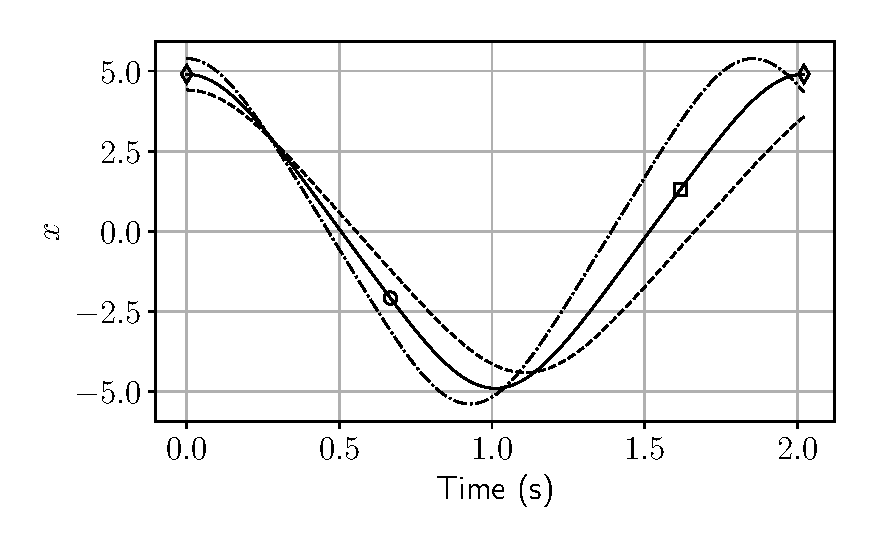
\includegraphics[width=\textwidth, height=5cm]{nnm/duff_per_time}
  \end{subfigure}
  ~
  \begin{subfigure}[b]{0.45\textwidth}
    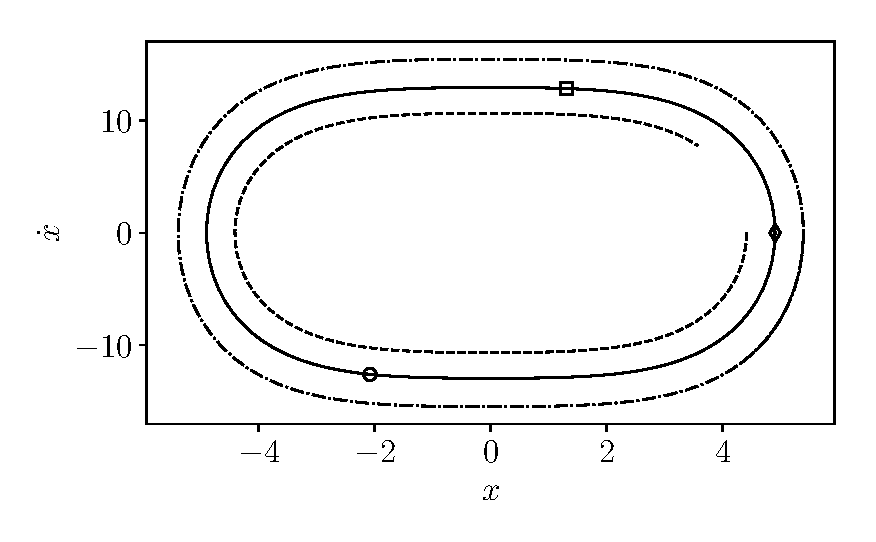
\includegraphics[width=\textwidth, height=5cm]{nnm/duff_per_space}
  \end{subfigure}
  \caption{Solution of the duffing eq. $\ddot x + x + 0.5x^3=0$ for different
    initial conditions and $T=2.0215$s.
    \textbf{(a)}: time series;
    \textbf{(b)}: phase space.
    Initial conditions for different line styles:
    \sampleline{}: [4.9009, 0];
    \sampleline{dashed}: 0.9$\cdot$[4.9009, 0];
    \sampleline{dotted}: 1.1$\cdot$[4.9009, 0];
    Markers represent different initial conditions for the periodic solution.
    $\diamond$: [4.9009, 0];
    $\square$: [1.308, 12.8764];
    $\circ$: [-2.0825, -12.6177]
  }
  \label{fig:sm_phase}
\end{figure}


In summary, the periodic solution is found by solving
\begin{equation}
  \label{eq:sm_bvp_problem}
  \bm h_{NNM} =
  \begin{bmatrix}
    \bm h(\bm z_{p}, T) \\
    g(\bm z_{p} )
  \end{bmatrix}
  = 0
\end{equation}

The solution is found by corrections to the initial guess, done by
Newton-Raphson iterations. The shooting function is expanded in a Taylor series
% around increments $\Delta \bm z_{p0}$ and $\Delta T_{p0}$

\begin{equation}
  \label{eq:sm_nr}
  \bm h +
  \bm h_{\bm z} \Delta \bm z_{p} +
  \bm h_{T} \Delta T
  + H.O.T. = 0
  % Jeg har glemt mixede product herunder:
  %\mathcal{O}(\Delta \bm z_{p0}^2, \Delta T_{p0}^2) = 0
\end{equation}
where all terms are evaluated at $(z_0,T)$ and $H.O.T.$ the neglected higher
order terms. Thus the corrections are found by solving the linear equation

\begin{equation}
  \label{eq:sm_nr_sol}
  \begin{bmatrix}
    \bm h_{\bm z} & \bm h_{T} \\
    g_{\bm z} & 0
  \end{bmatrix}
  \begin{bmatrix}
    \Delta \bm z_{p} \\
    \Delta T
  \end{bmatrix}
  = -
  \begin{bmatrix}
    \bm h \\
    g
  \end{bmatrix}
\end{equation}

Since $\bm h_{NNM}$ have the transformation $\mathbb{R}^{2n+1} \rightarrow
\mathbb{R}^{2n+1}$ the Newton system is over determined, ie. the matrix to
invert is not square and have to be solved in a least square sense.

The state is updated as

\begin{equation}
  \label{eq:sm_nr_update}
  \bm z^{k+1}_{p} = \bm z^k_{p} + \Delta \bm z^k_{p}, \quad
  T^{k+1} = T^k + \Delta T^k
\end{equation}
where $k$ is iteration number. The iteration is stopped when $\bm h_{nnm} = 0$
to some tolerance. Newmark-Raphson is a local algorithm, meaning that
convergence is guarantied when the initial guess is close to solution, otherwise
not. The initial guess is chosen as one the of linear mode shapes and
corresponding period. If the extended Jacobian matrix $\bm J = [\bm h_{\bm z},
\bm h_T] $ is exact, the convergence is second order.


The partial derivatives of the shooting function are found as:
\begin{align}
  \label{eq:sm_jac1}
  \bm h_{\bm{z}}&=
  \frac{\p \bm z(t; \bm z_0)}{\p \bm z_0}\bigg|_{t=T} - \bm I \\
  \bm h_T &=
  \frac{\p \bm z(t; \bm z_0)}{\p t}\bigg|_{t=T} =
  \bm h_{ham}(\bm z(T; \bm z_0))
  \label{eq:sm_jac2}
\end{align}
where $\bm h_{T}$ is a $2n$ vector, $\bm h_{\bm z_{0}}$ is $2n\times 2n$ matrix.


% The NR converges to a single solution depending on initial conditions. If
% It should be mentioned that for some forcing parameters, where a nonlinear
% system might have multiple solutions, the NR will, depending on the initial
% conditions, converge towards only one of them. Methods relying on the homotopy
% method or Groebner bases can be employed to find multiple solution - not that I
% know anything about these methods.

\subsubsection{Sensitivity analysis}
\label{sec:sm_sens_ana}

The Jacobian matrix $\p \bm z(t,\bm z_0) / \p \bm z_{0}$ from eq.
\eqref{eq:sm_jac2}, which represent the variation of the solution $\bm z(t,\bm
z_0)$ at time $t$ to pertubated initial conditions $\bm z_0$, is normally
calculated in two ways. Either by finite difference: successively pertubation of
each of the $2n$ initial condtion and integrating over the period. This is
computationally expensive and gives slower NR convergence since the Jacobi
matrix is only approximate.

Instead sensitivity analysis is used. The state space formulation
\eqref{eq:sm_state} is differentiated with respect to initial conditions $\bm
z_0$

\begin{align}
  &\frac{\p}{\p \bm z_0} \left[ \dot{\bm z}(t, \bm z_0) \right] =
    \frac{\p}{\p \bm z_0} \left[ \bm h_{ham}(\bm z) \right] \implies
  \nonumber \\
  &\frac{\d}{\d t} \left[  \frac{\p \bm z(t, \bm z_0)}{\p \bm z_0} \right] =
    \frac{\p \bm h_{ham}(\bm z)}{\p \bm z}\bigg|_{\bm z(t,\bm z_0)}
    \frac{\p \bm z(t, \bm z_0)}{\p \bm z_0}
    \label{eq:sm_sens}
\end{align}
with initial condition
\begin{equation}
  \label{eq:sm_sens_init}
  \frac{\p \bm z(0,\bm z_0)}{\p \bm z_0} = \bm I_{2n}
\end{equation}
since $\bm z(0;\bm z_0) = \bm z_0$.

Then eq. \eqref{eq:sm_sens} is integrated over $T$ to obtain the Jacobian matrix
at time $t=T$. This integration is linear and carried out at the same time as
the Newmark integration of the periodic solution. In practise the eom
formulation eq. \eqref{eq:per_eom} is used for the sensitivity analysis. See
appendix \ref{sec:newmark_sens} for a derivation. The sensitivity analysis
requires the nonlinear forces to be smooth. If they are nonsmooth, finite
difference have to be used.

\subsubsection{Marginal stability}
\label{sec:sm_stab}


For Hamiltonian systems the periodic solutions can at most be marginally stable
since the system is without damping. Thus without dissipation, nearby orbits are
not attracted to the periodic solution (ie. volume is conserved in phase plane),
but the orbit \textit{is} still stable.

The stability of a periodic solution is found from the Jacobian matrix evaluated
at $t=T$, called the \textit{monodromy matrix}

\begin{equation}
  \label{eq:sm_stab}
  \Phi = \frac{\p \bm z(t; \bm z_0)}{\p \bm z_0}\bigg|_{t=T}
\end{equation}

The stability is found from the eigenvalues $\sigma_i$ of $\Phi$, the Floquet
multipliers. If an Floquet multiplier is larger than one (i.e., $|\sigma_i|>
1$), the orbit is unstable. Conversely, the periodic orbit is stable if
$|\sigma_i| \leq 1, \forall i$

Equivalently the Floquet exponents $\lambda$ could be used. If there is at least
one Floquet exponents with a real part larger than 0 the solution is unstable.
They are related through,
\begin{equation}
  \label{eq:floquet_relations}
  \sigma_i = e^{\lambda_i T}
\end{equation}

Both variants are depicted on the complex plane and either compared to the unit
circle or the imaginary axis, respectively. See section \ref{sec:bifurcations},
fig \ref{fig:bifurcation} for a graphical representation.

It should be noted that for Hamiltonian systems, for marginally stable
solutions, the Floquet multipliers will always be complex conjugate pairs
\textit{on} the unit circle, not within as it is the case for asymptotically
stable solutions obtained from damped systems.
Further there is always one pair of eigenvalues at $(1,0)$, ie. where the x-axis
cross the unit circle in the complex plane. For Floquet exponents this means
that the a pair is always located at 0, expressed as $\max(\Re(\lambda)) = 0$.
This is due to the monodromy matrix of a Hamiltonian system being
\textit{symplectic} \autocite{steves2006a}.


\subsubsection{Damped and forced motion}

If the shooting method is used for damped and forced motion, only the state
space formulation have to be changed.

The state space formulated for the full eom \eqref{eq:per_eom} is

\begin{equation}
  \label{eq:app_state_space}
  \dot{\bm z}(t) = \bm L\bm z(t) - \bm g_{nl}(\bm z) + \bm g_{ext}(\omega,t)
\end{equation}
where

\begin{equation}
  \begin{aligned}
    \bm z =
    \begin{bmatrix}
      \bm x \\ \dot{\bm y}
    \end{bmatrix}, \quad
    \bm L =
    \begin{bmatrix}
      \bm 0 & \bm I_n \\
      -\bm M^{-1}\bm K & -\bm M^{-1} \bm C
    \end{bmatrix} \\
    \bm g_{nl} =
    \begin{bmatrix}
      \bm 0 \\ \bm M^{-1} \bm f_{nl}(\bm x, \dot{\bm x})
    \end{bmatrix}, \quad
    \bm g_{ext}
    \begin{bmatrix}
      \bm 0 \\ \bm M^{-1} \bm p_{ext}(\omega, t)
    \end{bmatrix}
  \end{aligned}
\end{equation}

Calculating the periodic motion for the full EOM, instead of the unforced and
undamped case, only requires changing the evaluation of the state space to the
formula above. The sensitivity analysis in section \ref{sec:newmark_sens} is
derived for the full EOM. Thus very few lines of code needs changing.


\subsection{Harmonic balance}
\label{sec:harmonic_bal}

Where the shooting method finds a periodic solution by solving the system in
time domain, HB finds the periodic solution in frequency domain. The method is
described by \textcite{detroux2016a}.

A periodic solution to the damped and forced eom eq. \eqref{eq:per_eom} is
sought.
As the displacements $\bm x$ and forces $\bm f(\bm x, \dot{\bm x}, \omega ,t) =
\bm p(\omega, t)- \bm f_{nl}(\bm x, \dot{\bm x})$ are assumed periodic, they are
approximated by Fourier series truncated to the $N_H$-th harmonic

\begin{align}
  \label{eq:hb_x_expansion}
  \bm x(t) &= \frac{\bm c^x_0}{\sqrt{2}} \sum_{k=1}^{N_H} (s^x_k \sin(k\omega t) +
          c^x_k \cos(k\omega t)) \\
  \label{eq:hb_f_expansion}
  \bm f(t) &= \frac{\bm c^f_0}{\sqrt{2}} \sum_{k=1}^{N_H} (s^f_k \sin(k\omega t) +
          c^f_k \cos(k\omega t))
\end{align}
where $\bm s_k$ and $\bm c_k$ represent the vectors of the Fourier coefficients
related to sine and cosine terms. The Fourier coefficients of the force $\bm f(t)$,
$\bm s^f_k$ and $\bm c^f_k$ depends on the Fourier coefficients of the
displacement $\bm x(t)$, $\bm s^x_k$ and $\bm c^x_k$ which are the new unknowns.
Gathering the coefficients into vectors

\begin{align}
  \label{eq:hb_coeffz}
  &\bm z =
    \begin{bmatrix}
      (\bm c^x_0)^T & (\bm s^x_1)^T & (\bm c^x_1)^T & \cdots &
      (\bm s^x_{N_H})^T & (\bm c^x_{N_H})^T
    \end{bmatrix}^T \\
  \label{eq:hb_coeffz}
  &\bm b =
    \begin{bmatrix}
      (\bm c^f_0)^T & (\bm s^f_1)^T & (\bm c^f_1)^T & \cdots &
      (\bm s^f_{N_H})^T & (\bm c^f_{N_H})^T
    \end{bmatrix}^T
\end{align}
then using a compact notion, the displacements and forces is written as

\begin{align}
  \label{eq:hm_x_compact}
  &\bm x(t) = (\bm Q(t) \otimes \bm I_n) \bm z \\
  \label{eq:hb_y_compact}
  &\bm f(t) = (\bm Q(t) \otimes \bm I_n) \bm b
\end{align}
where $\otimes$ is the Kronecker product and $\bm Q$ a vector with harmonic terms

\begin{equation}
  \label{eq:hb_Q}
  \bm Q(t) =
  \begin{bmatrix}
    \frac{1}{2} & \sin(\omega t) & \cos(\omega t) & \cdots & \sin(N_H \omega t) &
    \cos(N_H \omega t)
  \end{bmatrix}
\end{equation}

Velocities and accelerations are found using the Fourier series as
\begin{align}
  \label{eq:hb_vel}
  &\dot{\bm x} = \left( \dot{\bm Q}(t) \otimes \bm I_n \right) \bm z =
    \left( (\bm Q(t) \bm \nabla) \otimes \bm I_n \right) \bm z \\
  \label{eq:hb_acc}
  &\ddot{\bm x} = \left( \ddot{\bm Q}(t) \otimes \bm{I}_n \right) \bm z =
    \left( (\bm Q(t) \bm \nabla^2) \otimes \bm{I}_n \right) \bm z \\
\end{align}

By substituting eqs. \eqref{eq:hb_x_expansion}-\eqref{eq:hb_f_expansion} and
\eqref{eq:hb_vel}-\eqref{eq:hb_acc} into the eom \eqref{eq:per_eom} and using a
galerkin procedure, one ends up with the equations of motion in frequency
domain (see appendix \ref{sec:hb_appendix} for more details on the derivation
and definition of $\bm \nabla$(the gradient as diagonal matrix))

\begin{equation}
  \label{eq:hb_feom}
  (\bm \nabla^2 \otimes \bm M)\bm z + (\bm \nabla \otimes \bm C)\bm z +
  (\bm{I}_{2N_H} \otimes \bm K)\bm z =
  (\bm{I}_{2N_H} \otimes \bm{I}_n )\bm b
\end{equation}
or in more compact form

\begin{equation}
  \label{eq:hb_feom_compact}
  \bm h(\bm z, \omega) = \bm A(\omega) \bm z - \bm b(\bm z) = \bm 0
\end{equation}
where $\bm A$ describes the linear dynamics

\begin{equation}
  \label{eq:hb_A}
  \bm A = \bm \nabla^2 \otimes \bm M + \bm \nabla \otimes \bm C +
  \bm{I}_{2N_H} \otimes \bm K
\end{equation}

If $\bm z$ is a solution of \eqref{eq:hb_feom_compact}, then the time signal
$\bm x$ constructed from $\bm z$ is periodic and satisfies the eom
\eqref{eq:per_eom}. As with the shooting function, eq.
\eqref{eq:hb_feom_compact} is nonlinear (due to $\bm b$ dependence on $\bm z$)
and have to be solved iterative by Newton-Rahpson iterations. It should
however be noted that $\bm h(\bm z, \omega)$ is an (nonlinear) algebraic
equation, ie. there is no need for time integration. The increments are found as

\begin{equation}
  \label{eq:hb_nr}
  \bm z^{(k+1)} = \bm z^{(j)} -
  \frac{\bm h(\bm z, \omega)}{\bm h_{\bm z}(\bm z, \omega)}
\end{equation}


\subsubsection{Expression of nonlinear terms and Jacobian matrix}
\label{sec:hb_exp_nonlin_jac}

Solution of eq \eqref{eq:hb_nr} requires calculation of $\bm h$ and of the
Jacobian matrix $\bm h_{\bm z}$, which in turn requires calculation of $\bm b$
and its derivatives.

It is not known how the Fourier coefficients in $\bm b$ relates to the
coefficients in $\bm z$, ie. it is not possible to directly calculate $\bm b(\bm
z)$ due to $\bm f_{nl}$ depends on $\bm x$. Instead a technique called the
\textit{alternating frequency-time domain}(AFT) method is used. Here $\bm b$ is
calculated through successive Fourier transformations as shown in figure
\ref{fig:hb_aft}

\begin{center}
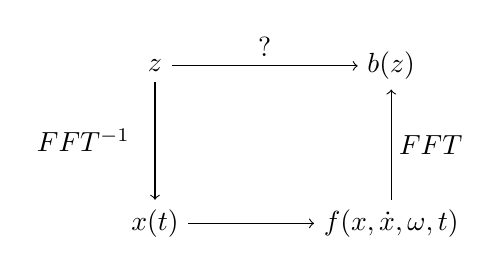
\begin{tikzpicture}[node distance=1.5cm]
  % nodes
  \node (A) at (0, 2) {$\bm z$};
  \node (B) at (0, 0) {$\bm x(t)$};
  \node (C) at (3, 0) {$\bm f(\bm x,\dot{\bm x},\omega, t)$};
  \node (D) at (3, 2) {$\bm b(\bm z)$};
  % arrows
  \draw [->]
  (A) edge node[anchor=center, text width=3.0cm] {$FFT^{-1}$} (B)
  (B) edge (C)
  (C) edge  node[anchor=center, text width=-0.2cm] {$FFT$} (D)
  (A) edge  node[anchor=center, above] {?} (D);
\end{tikzpicture}
\captionof{figure}{Graphical representation of the alternating frequency-time
  domain (AFT) method}
\label{fig:hb_aft}
\end{center}

$\bm x$ is calculated from the Fourier coefficients in $\bm z$, then the
nonlinear (and external) forces $\bm f$ are evaluated in time domain and $\bm b$
is found as the Fourier coefficients of $\bm f$.

The Jacobian matrix is given by
\begin{equation}
  \label{eq:hb_jac1}
    \bm h_{\bm z} = \frac{\p \bm h}{\p \bm z} = \bm A - \frac{\p \bm b}{\p \bm z}
\end{equation}
where the hard part is to compute $\bm b_{\bm z}$. The method for calculating
the Jacobian matrix (explicit $\bm b_{\bm z}$) follows the AFT method as well.
To do that, the inverse Fourier transform is written as the linear operator $\bm
\Gamma(\omega)$

\begin{equation}
  \label{eq:hb_gamma}
  \begin{aligned}
    \bm \Gamma(\omega) =
    \left[
  \begin{matrix}
    \bm{I}_n \otimes
    \begin{bmatrix}
      1/\sqrt{2} \\ 1/\sqrt{2} \\ \vdots \\ 1/\sqrt{2}
    \end{bmatrix} &
    \bm{I}_n \otimes
    \begin{bmatrix}
      \sin(\omega t_1) \\ \sin(\omega t_2) \\ \vdots \\ \sin(\omega t_{t_N})
    \end{bmatrix} &
    \bm{I}_n \otimes
    \begin{bmatrix}
      \cos(\omega t_1) \\ \cos(\omega t_2) \\ \vdots \\ \cos(\omega t_{t_N})
    \end{bmatrix}&
        \cdots
  \end{matrix}
\right. \\
\left.
  \begin{matrix}
    \bm{I}_n \otimes
    \begin{bmatrix}
      \sin(N_H\omega t_{}) \\ \sin(N_H\omega t_2) \\ \vdots \\ \sin(N_H\omega t_{t_N})
    \end{bmatrix} &
    \bm{I}_n \otimes
    \begin{bmatrix}
      \cos(N_H\omega t_{}) \\ \cos(N_H\omega t_2) \\ \vdots \\ \cos(N_H\omega t_{t_N})
    \end{bmatrix}
  \end{matrix}
\right]
\end{aligned}
\end{equation}

which is used on the concatenated time series
\begin{equation}
  \label{eq:hb_time_series}
  \begin{aligned}
    \tilde{\bm x} =
    \begin{bmatrix}
      x_1(t_1) & \cdots & x_1(t_N) & \cdots & x_n(t_1) & \cdots & x_n(t_N)
    \end{bmatrix}^T\\
    \tilde{\bm f} =
    \begin{bmatrix}
      f_1(t_1) & \cdots & f_1(t_N) & \cdots & f_n(t_1) & \cdots & f_n(t_N)
    \end{bmatrix}^T
  \end{aligned}
\end{equation}

Thus the inverse and direct Fourier transform are written
\begin{equation}
  \label{eq:hb_four_transform}
    \tilde{\bm x} = \bm \Gamma(\omega) \bm z, \quad
    \bm z =( \bm \Gamma(\omega))^+ \tilde{\bm x}
\end{equation}
where $()^+$ is the Moore-Penrose pseduinverse and used as $\Gamma$ is not
square. In implementation the solution is found by a least square solver.

The Fourier coefficients of the external and nonlinear forces are then
\begin{equation}
  \label{eq:hb_b_coeff}
  \bm b(\bm z) = ( \bm \Gamma(\omega))^+ \tilde{\bm f}
\end{equation}
and the Jacobian is computed as
\begin{equation}
  \label{eq:hb_jac}
  \bm h_{\bm z} = \bm A - \frac{\p \bm b}{\p \bm z} =
  \bm A -
  \frac{\p\bm b}{\p \tilde{\bm f}}
  \frac{\p \tilde{\bm f}}{\p \tilde{\bm x}}
  \frac{\p \tilde{\bm x}}{\p \bm z} =
  \bm A - \bm \Gamma^+ \frac{\p \tilde{\bm f}}{\p \tilde{\bm x}} \bm \Gamma
\end{equation}

It should be noted that the concatenated time series vectors $\tilde{\bm x}$ and
$\tilde{\bm f}$ are newer used. They are only used in the derivation for the
expression for the Jacobian. Only the Fourier operator $\bm \Gamma$ and
extracted Fourier coefficients $\bm x$ are used.


\subsubsection{Stability}
\label{sec:hb_stab}

Unlike the shooting method (or general time domain methods), the monodromy
matrix is not readily available as a byproduct since there is no time
integration. Instead for frequency methods, \textit{Hills method} is used to
approximate the Floquet exponents by solving a quadratic eigenvalue problem
whose components are obtained as byproduct of the HB method.

Perturbing a periodic solution by an exponential decay
\begin{equation}
  \label{eq:hb_pert}
  \bm p(t) = \bm x(t) + e^{\lambda t}\bm s(t)
\end{equation}
and inserting this into the eom eq. \eqref{eq:per_eom} it is shown in appendix
\ref{sec:hb_stab_appendix} that the quadratic eigenvalue problem is found as

\begin{equation}
  \label{eq:hb_quad_eigen}
  \bm \Delta_2 \bm \lambda^2 + \bm \Delta_1 \bm \lambda + \bm h_{\bm z} = \bm 0
\end{equation}
where $\bm \Delta$ are matrices describing the linear dynamics similar to $\bm
A$ in eq. \eqref{eq:hb_A} and $\lambda$ are Hills coefficients.

The quadratic eigenvalue problem is rewritten to a linear eigenvalue problem of
double size

\begin{equation}
  \label{eq:hb_double_eigen}
  \bm B_1 - \gamma \bm B_2 = \bm 0
\end{equation}
where

\begin{equation}
  \label{eq:hb_stab_B12}
  \bm B_1 =
  \begin{bmatrix}
    \bm \Delta  & \bm h_{\bm z} \\
    -\bm{I}    & \bm 0
  \end{bmatrix}, \quad
  \bm B_2 = -
  \begin{bmatrix}
    \bm \Delta_2   & \bm 0 \\
    \bm 0          & \bm{I}
  \end{bmatrix}
\end{equation}

The coefficients $\bm \lambda$ are found as the eigenvalues of the $(2N_H+1)2n$
square matrix

\begin{equation}
  \label{eq:hb_B}
  \bm B = \bm B^{-1}_2 \bm B_1 =
  \begin{bmatrix}
    -\bm \Delta^{-1}_2 \bm\Delta_1 & -\bm \Delta^{-1}_2 \bm h_{\bm z} \\
    \bm{I}                    & \bm 0
  \end{bmatrix}
\end{equation}
or from the generalised eigenvalueproblem eq. \eqref{eq:hb_double_eigen}

Only $2n$ eigenvalues approximate the Floquet exponents $\tilde{\bm \lambda}$,
the rest are spurious. The ones needed are the $2n$ values with smallest
imaginary magnitude.

The diagonal matrix
\begin{equation}
  \label{eq:hb_B_tilde}
  \tilde{\bm B} =
  \begin{bmatrix}
    \tilde \lambda_1 \\
    & \ddots \\
    & & \tilde \lambda_{2n}
  \end{bmatrix}
\end{equation}
gathers the Floquet exponents identified from the $(2 N_H + 1)2n$ Hill's
coefficients. Besides stability, they are used for detecting bifurcations in
section \ref{sec:detecting_bifs}.

\subsubsection{Example}
\label{sec:hb_example}

Figure \ref{fig:hb_duffing_periodic} shows the periodic of the coupled duffing
Duffing system. Although the excitation is pure sine, the response contains
multiple harmonics due to the nonlinearity.
As the fifth harmonic only participates marginally, it can be assumed that
even higher harmonics are not important for describing the periodic motion.
The number of harmonic participating, and their weights, depends on the forcing
frequency and the level of nonlinearity(ie. including the forcing level).

The normalised harmonic components are found as

\begin{equation}
  \label{eq:hb_normal_coeff}
  \begin{aligned}
    \sigma_i = \frac{\phi_i}{\sum_{k=0}^{N_H} \phi_i}, \quad (i=0,\cdots, N_H) \\
    \phi_0 = \frac{c_0^x}{\sqrt{2}}, \quad \phi_i = \sqrt{(s^x_i) + (c^x_i)^2}
  \end{aligned}
\end{equation}


\begin{figure}[!ht]
  \centering
  \begin{subfigure}[b]{0.6\textwidth}
    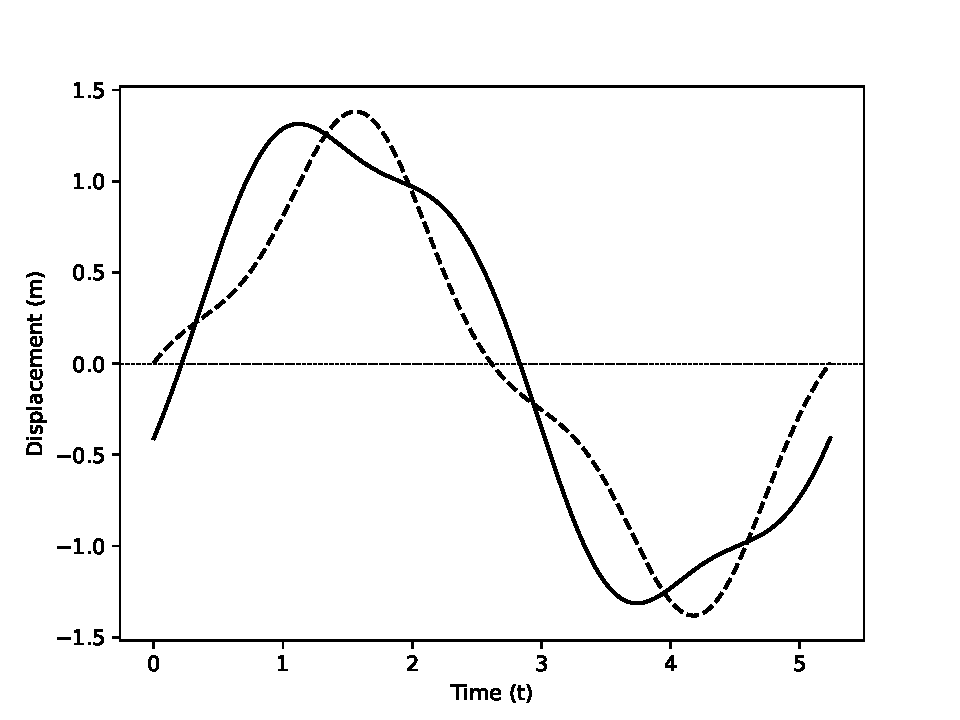
\includegraphics[width=\linewidth, height=6cm]{2dof_duffing/hb_per}
    \caption{}
  \end{subfigure}
  ~
  \begin{subfigure}[b]{0.36\textwidth}
    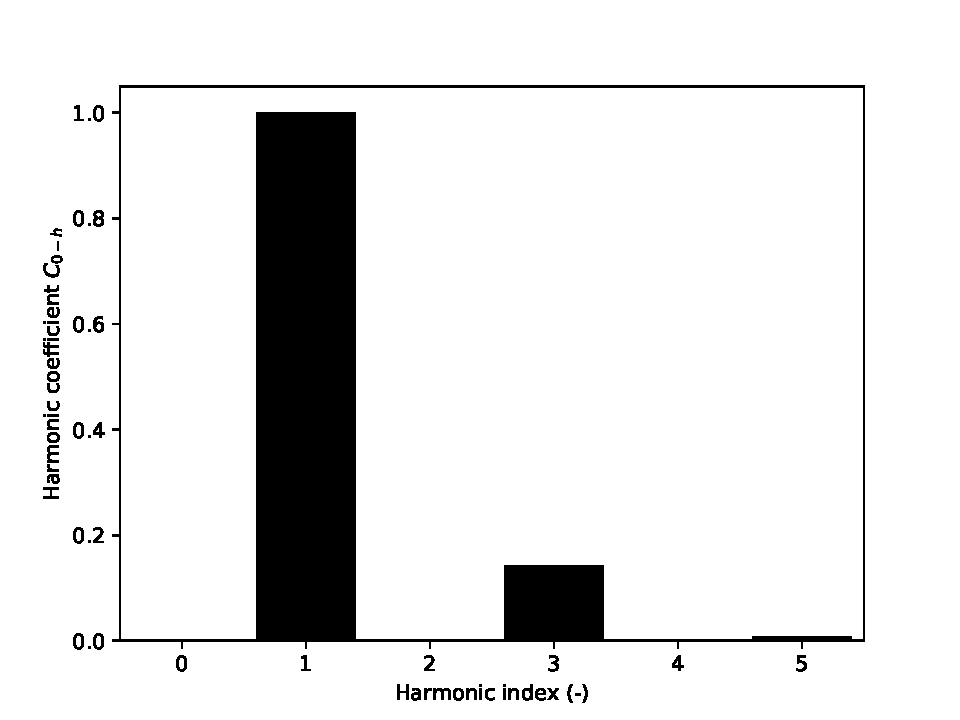
\includegraphics[width=\linewidth, height=6cm]{2dof_duffing/hb_har}
    \caption{}
  \end{subfigure}
  \caption{Periodic solution of the coupled Duffing system \eqref{eq:2dof} for
    $f=2$N,
    $\omega=1.2$rad/s and $N_H=5$.
    \textbf{(a)}: Time series.
    \sampleline{}: $x_1$,
    \sampleline{dashed}: $x_2$;
    \textbf{(b)}: Normalized harmonic components of $x_1$.}
  \label{fig:hb_duffing_periodic}
\end{figure}
\FloatBarrier

\subsection{Summary}
\label{sec:per_summary}

Periodic solutions of nonlinear structures can be computed with
time-domain(shooting method) and frequency-domain(harmonic balance) methods. The
main difference is in the implementation complexity, computional complexity and
accuracy. Both methods can be used together with continuation and have ways to compute
stability analysis without much extra cost.

Summarising the shooting method
\begin{multicols}{2}
  Pro
  \begin{itemize}
  \item Accurate
  \item (all) Higher harmonics represented
  \end{itemize}
  \columnbreak
  Cons
  \begin{itemize}
  \item Many time integrations
  \item Slow for larger systems
  \end{itemize}
\end{multicols}


Summarising the harmonic balance method
\begin{multicols}{2}
  Pro
  \begin{itemize}
  \item Fast
  \item Harmonic coefficients available
  \item Can be used for filtering, ie. by defining the number of harmonics in
    the solution.
  \end{itemize}
  \vfill\null
  \columnbreak
  Cons
  \begin{itemize}
  \item Less accurate
  \item High number of harmonic might be necessary. Need to check the
    contribution from last harmonics to ensure enough is included.
  \end{itemize}
\end{multicols}


Stability of a periodic solution can be assessed through  their Floquet
multipliers or exponents. When the Shooting method is used, they are found from
the monodromy matrix. When HB is used, they are found from Hills matrix.


%%% Local Variables:
%%% mode: latex
%%% TeX-master: "../../report"
%%% End:
